\subsection{Final Result}

\begin{frame}
      \begin{theorem}
            \begin{equation}
                  \theta(C_{n}) \leq \sqrt{5}
            \end{equation}
      \end{theorem}
\end{frame}

\begin{frame}
      \begin{proof}
            Consider an umbrella that has a handle and $5$ ribs that all have unit length. And also its handle is a unit vector.

            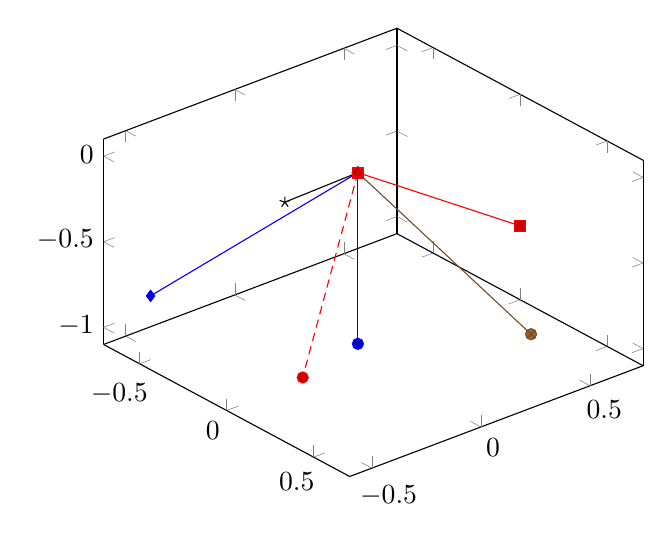
\begin{tikzpicture}
                  % TODO add label to point

                  \begin{axis}[view = {50}{40}]
                        
                  \addplot3 coordinates 
                  {
                        (0,0,0)
                        (0,0,-1)
                  };

                  \addplot3 coordinates 
                  {
                        (0,0,0)
                        (0,0.74349606,-0.66874031)
                  };
                        
                  \addplot3 coordinates 
                  {
                        (0,0,0)
                        (0.70710677,0.22975292,-0.66874031)
                  };

                  \addplot3 coordinates 
                  {
                        (0,0,0)
                        (-0.70710677,0.22975292,-0.66874031)
                  };


                  \addplot3 coordinates 
                  {
                        (0,0,0)
                        (-0.43701602,-0.60150095,-0.66874031)
                  };
                  
                  \addplot3 coordinates 
                  {
                        (0,0,0)
                        (0.43701602,-0.60150095,-0.66874031)
                  };

                  \end{axis}
                        
            \end{tikzpicture}

      \end{proof}
\end{frame}

\begin{frame}
      \begin{proof}
            Here, angles between two consecutive ribs are same. 
            
            Let $v$ be a rib. And let $w$ be one of the rib that have the largest angle with $v$. Then, we let the angle between $v$ and $w$ be $ \pi/2 $.

            Then, the $5$ ribs of such an umbrella form an orthonormal representation of $C_{5}$.

            Let $d$ be the vector represent the handle, and $v_{1},v_{2},\dots,v_{5}$ be the $5$ ribs. And let $\gamma$ be the angle between the handle and any rib.

            So, by some calculation, we get
            \begin{eqnarray}
                  \theta(C_{5}) &\le& \max \frac{1}{<d,v_{i}>^{2}} \\
                  &=& \left(
                        \frac{1}{\cos(\gamma)}
                  \right)^{2} \\
                  &=& \sqrt{5}
            \end{eqnarray}
      \end{proof}
\end{frame}